\documentclass[letterpaper]{article}

% if you need to pass options to natbib, use, e.g.:
% \PassOptionsToPackage{numbers, compress}{natbib}
% before loading nips_2017
%
% to avoid loading the natbib package, add option nonatbib:
% \usepackage[nonatbib]{nips_2017}

\usepackage[final]{nips_2017}

% to compile a camera-ready version, add the [final] option, e.g.:
% \usepackage[final]{nips_2017}

\usepackage[utf8]{inputenc} % allow utf-8 input
\usepackage[T1]{fontenc}    % use 8-bit T1 fonts
\usepackage{hyperref}       % hyperlinks
\usepackage{url}            % simple URL typesetting
\usepackage{booktabs}       % professional-quality tables
\usepackage{amsfonts}       % blackboard math symbols
\usepackage{nicefrac}       % compact symbols for 1/2, etc.
\usepackage{microtype}      % microtypography\\

\usepackage{amsmath, amsthm, graphicx, bbm, color, mathtools}
\usepackage{algpseudocode, algorithm, algorithmicx}

\makeatletter
\def\BState{\State\hskip-\ALG@thistlm}
\makeatother

\DeclareMathOperator*{\argmin}{arg\,min}
\DeclareMathOperator*{\argmax}{arg\,max}
\numberwithin{equation}{section}
\theoremstyle{plain}
\newtheorem{theorem}{Theorem}[section]
\newtheorem{lemma}{Lemma}[section]

\title{Optimal betting for a multi-armed bandit}

% The \author macro works with any number of authors. There are two
% commands used to separate the names and addresses of multiple
% authors: \And and \AND.
%
% Using \And between authors leaves it to LaTeX to determine where to
% break the lines. Using \AND forces a line break at that point. So,
% if LaTeX puts 3 of 4 authors names on the first line, and the last
% on the second line, try using \AND instead of \And before the third
% author name.

\author{
  Kurt~Ehlert\\
  \texttt{kehlert@math.wisc.edu}\\
  %% examples of more authors
  %% \And
  %% Coauthor \\
  %% Affiliation \\
  %% Address \\
  %% \texttt{email} \\
  %% \AND
  %% Coauthor \\
  %% Affiliation \\
  %% Address \\
  %% \texttt{email} \\
  %% \And
  %% Coauthor \\
  %% Affiliation \\
  %% Address \\
  %% \texttt{email} \\
  %% \And
  %% Coauthor \\
  %% Affiliation \\
  %% Address \\
  %% \texttt{email} \\
}

\begin{document}
% \nipsfinalcopy is no longer used

\maketitle

\begin{abstract}
If we are betting on a slot machine, then the natural question to ask is ``how much should we bet''? If the probability of winning is $p$, it turns out that betting a fraction of our wealth equal to $2p-1$ is an optimal strategy in many senses. However, if we are faced with many slot machines with unknown probabilities of winning, then how should we bet, and which slot machines should we bet on? We will present the Kelly-UCB algorithm, which addresses this more complicated problem. We will also provide analytic and numerical results regarding the performance of the Kelly-UCB algorithm.
\end{abstract}

\section{Introduction}
A slot machine is also known as a one-armed bandit, because early slot machines were operated by pulling a lever (arm) attached to their side \citep{onearmedbanditdict}. Suppose that we are pulling an arm with a probability $p$ of winning, where $\nicefrac{1}{2} < p < 1$. Also, we start with a finite amount of money, and we can bet any fraction of our wealth each time we pull the arm. We win an amount equal to our bet with probability $p$, and conversely we lose our bet with probability $1-p$. If $p > 1/2$, then we are likely to gain money by playing the game, but we need to be careful with our betting strategy. If we bet a fraction of our wealth equal to $2p-1$, then this strategy is known as the ``Kelly bet'' \citep{kelly1956new,thorp2006kelly}. In some senses it maximizes our wealth, and it also avoids bankruptcy. In Section \ref{singlearmed}, we briefly discuss the Kelly bet for a slightly generalized situation and prove that it is optimal in a few basic senses.

Now consider a situation where we can choose between many arms. If we pull arm $i$, then we win with probability $p_i$ and lose with probability $1-p_i$. If we are only allowed to bet a fixed amount and we do not know the value of $p_i$ for any $i$, then this is called the stochastic multi-armed bandit problem. There is a trade-off between exploitation and exploration: we want to exploit an arm with a seemingly high probability of winning, but we also want to explore and find the best arm. Here we consider a new version of the stochastic bandit problem. Instead of fixed-size bets, we can bet any fraction of our wealth. The KL-UCB algorithm in \cite{cappe2013kullback} does not address how much to bet, so we plan to extend the KL-UCB algorithm and its analysis to the variable-bet situation. We will also allow for more complicated payoffs than just a win or loss of our entire bet.

In Section \ref{singlearmed}, we review the Kelly bet for the one-armed bandit with known probabilities. Then we extend the Kelly bet to the situtation where we do not know the probabilities of the possible outcomes. Section \ref{mab} outlines our Kelly-UCB algorithm for playing a variable-bet multi-armed bandit. Then we will present analytic and numerical results on the algorithm's performance.

\section{Optimal betting for a single-armed bandit}\label{singlearmed}
\subsection{Kelly bet for a bandit with a known probability of winning}
Suppose we are playing a slot machine that allows us to bet any proportion of our wealth. Let $X_n$ be a random variable that takes on only finitely many values in $[-1,\infty)$.  When we pull the arm, we obtain of profit of $X_n$ per unit bet on the $n^\text{th}$ pull. For example, if we bet \$100 and $X_1 = -1$, then we lose our entire bet of \$100. If instead $X_1 = 2$, then we win \$200 (and get back our original bet pf \$100). Let $p_j$, $1\le j \le m$, denote the probability that $X_n$ is equal to $x_j$. Furthermore, assume that $p_j$ is known for every $j$, the $X_n$ are i.i.d., and that $\mathbb{E}[X_1] > 0$. Also assume that $P(X_1 = -1) > 0$.

If we want to maximize our expected gain, then we should bet our entire fortune on every pull, but we would go bankrupt with probability $1$. If we bet a fixed amount, then there is still a positive probability of going bankrupt. Instead we will take a different approach and bet a fixed proportion of our wealth on each pull. Later we will show that this is actually optimal in two senses. \cite{ethier2010doctrine} analyzes the Kelly bet in much more detail and shows that it is optimal in many more ways than we consider here. \cite{ethier2010doctrine} also notes that some of the assumptions on $X_1$ can be relaxed, namely it does not need to be discrete-valued and we can have $P(X_1 = -1) =0$.

Let $W_0$ be our initial wealth, and let $W_n$ is our wealth after pull $n$. Define $f$ as the proportion of our wealth that we bet. Then
\begin{align}
W_n &= W_{n-1} +fW_{n-1} X_n\\
&= W_{n-1} (1+fX_n)
\end{align}
Using recursion, we can see that our wealth after pull $n$ is
\begin{equation}
W_n = W_0 \prod_{i=1}^n (1+f X_i)
\end{equation}
Let $r_n(f) = n^{-1} \log (W_n / W_0)$, then we can trivially rewrite our wealth after pull $n$ as
\begin{equation}
W_n = W_0 e^{r_n(f) n}
\end{equation}
We can interpret $r_n$ as the average geometric growth rate of our wealth after pull~$n$. Intuitively, we want to maximize the growth rate of our wealth. That intuition leads to the following lemma, which is based on Lemma 10.1.1 in \cite{ethier2010doctrine}
\begin{lemma}\label{kelly_asymp_growth}
Let $\mu(f) = \mathbb{E}[\log(1+fX_1)]$, which is defined for $f\in[0, 1)$. Then $\lim_{n\to\infty} r_n(f) = \mu(f)$. Let $f^* = \argmax_{0\le f\le 1} \mu(f)$, then $\mu(f^*) > 0$.
\end{lemma}
\begin{proof}
The strong law of large numbers implies
\begin{equation}
\lim_{n\to\infty}  r_n(f) = \lim_{n\to\infty} \frac{1}{n} \sum_{i=1}^n \log(1+f X_i) = \mathbb{E}[\log(1+fX_1)] \text{ a.s.}
\end{equation}
$\mu(f)$ is strictly concave, because
\begin{equation}
\mu''(f) = -\mathbb{E}\left[\frac{X^2}{(1+fX)^2}\right] < 0
\end{equation}
Therefore we can find the global maximum of $\mu(f)$ by just setting its derivative equal to 0. If $P(X_n = 1) = 1-P(X_n=-1)$, then $\mu'(f)$ is straightforward to compute and we find that $\argmax_{0\le f\le 1}\mu(f) = 2p-1$. Furthermore, $\mu'(0) =\mathbb{E}[X] > 0$, and $P(X_1 = -1 > 0)$ implies that $\mu'(1^-) = -\infty$. Therefore $\mu'(f) = 0$ for some $f$. Since $\mu(f)$ is strictly concave, there is a unique $f$ that satisfies $\mu'(f) = 0$ and maximizes $\mu(f)$.. Denote that $f$ as $f^*$. Furthermore, since $\mu(0) = 0$ and $\mu'(0) > 0$, we must have $\mu(f) > 0$ for some small enough $f$ near 0. Consequently, $\mu(f^*) > 0$.
\end{proof}
This fixed-proportion betting system is known as the \textit{Kelly bet} or \textit{Kelly criterion} \citep{kelly1956new,thorp2006kelly}. Above we showed that the Kelly bet is optimal in an asymptotic sense, so the natural question to ask is if it is also optimal for finite times. If we wish to maximize the logarithm of our wealth after $n$ pulls, then once again the Kelly bet is optimal.
\begin{lemma}
$f^*$ maximizes $\mathbb{E}[\log W_n(f)]$.
\end{lemma}
\begin{proof}
From the definition of $W_n$ and the linearity of expectations
\begin{align}
\mathbb{E}[\log W_n(f)] &= \log W_0 + \sum_{i=1}^n \mathbb{E}[\log (1+f X_n)]\\
&= \log W_0 + n \mu(f)
\end{align}
Therefore maximizing the log-wealth is equivalent to maximizing $\mu(f)$. In lemma \ref{kelly_asymp_growth} we showed that $f = 2p-1$ maximizes $\mu(f)$.
\end{proof}

The Kelly bet also approximately maximizes the median wealth. Also, in the long-run it will do better than any other ``essentially different'' strategy, which includes strategies that change betting proportions between pulls. \cite{ethier2010doctrine} provides the details.

\subsection{Kelly bet for a bandit with an unknown probability of winning}\label{kelly_unknown_prob}
A simple approach to estimating the Kelly bet would be to calculate $f^*$ based on estimated values of $\{p_j\}_{j=1}^m$. The obvious estimators are
\begin{equation*}
\bar{p}_j = \frac{1}{n} \sum_{i=1}^n \mathbbm{1}(X_i = x_j),\,1\le j\le m
\end{equation*}
This approach is not unreasonable, because our wealth would generally grow if $\bar{p}$ is close to to the actual probability of winning $p$. However, we would likely go bankrupt during the first few pulls, since $\bar{p}$ has a relatively high probability of being $\pm 1$. A reasonable idea is to shrink $f_n$ toward zero. \cite{orabona2016coin} show that by using the \cite{krichevsky1981performance} (KT) estimate of $p$, then our bets converge to the Kelly bet while controlling our losses. The KT estimate of $f_n$ essentially shrinks $f_n$ toward 0. The KT estimator of $p$ is
\begin{equation}
\hat{p}_n = \frac{1}{n+1}\left(\frac{1}{2} + \sum_{i=1}^n \mathbbm{1}\{X_i = 1\} \right)
\end{equation}
Let $\hat{f}_n=2\hat{p}_n-1$ be our bet on pull $n$, then
\begin{equation}
\hat{f}_n = 2\hat{p}_n-1 = \frac{1}{n+1}\sum_{i=1}^n X_i
\end{equation}
Thus our wealth after pull $n$ is
\begin{equation}
W_n = W_0\prod_{i=1}^n 1+f_i X_i
\end{equation}
Define $f_i$ and $p_i$ such that $f_i = 2p_i - 1$. Also let $Y_i = (1+X_i)/2$, and define the loss $\ell(p_i,Y_i)$ as
\begin{equation}\label{ell_loss}
\ell(p_i,Y_i) = -x_i\log p_i - (1-Y_i)\log(1-p_i)
\end{equation}
Combining the above definitions leads to the following
\begin{align}
\log W_n &= \log W_0 + \sum_{i=1}^n \log(1+f_i X_i)\\
&= \log W_0 + \sum_{i=1}^n \frac{1+X_i}{2} \log(2 p_i) + \frac{1-X_i}{2}\log(2(1-p_i))\\
&= \log W_0 + n\log 2 + \sum_{i=1}^n \frac{1+X_i}{2}\log(p_i) + \frac{1-X_i}{2}\log(1-p_i)\\
&= \log W_0 + n\log 2 - \sum_{i=1}^n \ell(p_i,Y_i)
\end{align}
Since the above holds for any choice of $p_i$, in particular it holds for $p_i=p,\hat{p}_n$. Let $W_n^*$ be our wealth from using the Kelly bet ,and let $W_n^\circ$ be our wealth using $\hat{p}_i$, where the $\hat{p}_i$ are $\sigma(X_1,X_2,\ldots,X_{i-1})$ measurable. Define the regret $R_n$ as
\begin{equation}
R_n = \log W_n^* - \log W_n^\circ = \sum_{i=1}^n \ell(\hat{p}_i,Y_i) - \ell(p,Y_i)
\end{equation}

Let $n_1 = \sum_{i=1}^n \mathbbm{1}\{X_i=1\}$, then according to \cite{cesa2006prediction} the KT estimator satisfies
\begin{equation}
R_n = \log\frac{\pi p^{n_1}(1-p)^{n-n_1}}{\text{Beta}(n_1+\nicefrac{1}{2}, n-n_1 + \nicefrac{1}{2})}
\end{equation}
The right-hand side of the above expression attains its maximum at $n_1 = np$. Therefore we have the following bound
\begin{equation}
R_n \le -nH(p) -\log \text{Beta}(np+\nicefrac{1}{2}, n(1-p)+\nicefrac{1}{2}) + \log(\pi)
\end{equation}
If $np$ is an integer, then the bound is sharp. We can use Stirling's formula to approximate the beta function, which gives
\begin{align}\label{kt_regret_bound}
R_n &\le -nH(p) -\log \text{Beta}(np+\nicefrac{1}{2}, n(1-p)+\nicefrac{1}{2}) + \log(\pi)\\
&\sim \frac{1}{2}\log(n+1) + \frac{1}{2}\log(\pi/2) + o(1)\label{asymp_regret_bound}
\end{align}

\begin{figure}[ht]
\centering
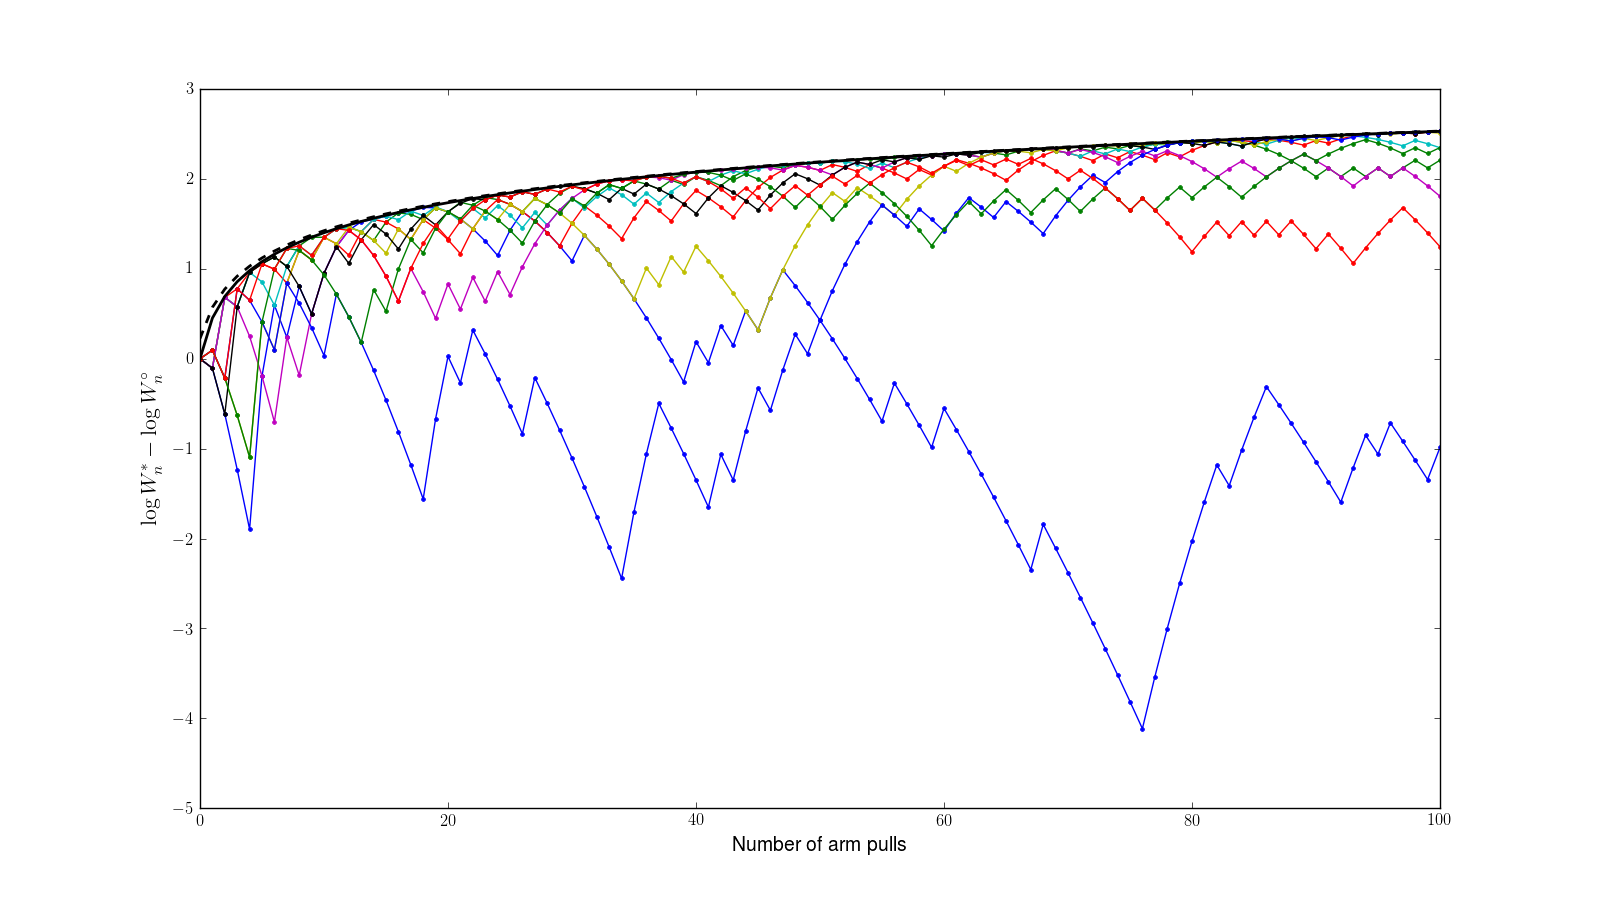
\includegraphics[width=0.9\textwidth]{single_arm_kt_regret.png}
\caption{Comparison of regret paths to the KT regret bound for $p=0.55$. The bold black curve on top is the regret bound $-nH(p) -\log \text{Beta}(np+\nicefrac{1}{2}, n(1-p)+\nicefrac{1}{2}) + \log(\pi)$ from \eqref{kt_regret_bound}. The dashed black curve is the asymptotic bound \eqref{asymp_regret_bound}. The others plots are the regrets of ten different paths.}
\label{single_arm_regret_figure}
\end{figure}

\section{Kelly-UCB algorithm for a multi-armed bandit}\label{mab}
In this section, we consider a situation where we have a choice between many different arms. If we pull arm $i$, then we win with probability $p_i$ and lose with probability $1-p_i$. If we are only allowed to bet a fixed amount and we do not know the value of $p_i$ for any $i$, then this is called the stochastic multi-armed bandit problem. There is a trade-off between exploitation and exploration: we want to exploit an arm with a seemingly high probability of winning, but we also want to explore and find the best arm.

There are many variations of the multi-armed bandit problem described in \cite{bubeck2012regret}. Here we consider a new version of the stochastic bandit problem. Instead of fixed-size bets, we can bet any fraction of our wealth. The KL-UCB algorithm in \cite{cappe2013kullback} decides which arms to pull, but it does not address how much to bet. We also want to allow ``shorting'', which means that we gain our bet if a pull is a loss (i.e. bet negative amounts). We modified the KL-UCB algorithm to allow for variable bets and shorting.

\subsection{Description of the Kelly-UCB algorithm}
Suppose there are $K$ levers that are indexed by $i=1,\ldots, K$. At each time $t=1,2,\ldots$, we can choose which lever to pull. Let $\{X_{i,t}\}$ be independent random variables indicating the payoff of lever $i$ on pull $t$, where $P(X_{i,t}=1) = 1-P(X_{i,t}=-1) = p_i$. We also need to decide how much to bet. We start with a finite amount of wealth, and we stop betting if we go bankrupt.

Let $W_0$ be our initial wealth, and let $f_{i,t}$ be the fraction of our wealth we bet on lever $i$ at time $t$. Also let $I_t\in\{1,\ldots,K\}$ be the index of the lever we pull at time $t$. Then
\begin{equation}\label{eq:wealth_def}
W_T = W_0 \prod_{t=1}^T (1+f_{I_t, t}X_{I_t,t})
\end{equation}
Below is the Kelly-UCB algorithm. Note that our lever choice is given by a modified version of the KL-UCB algorithm in \cite{cappe2013kullback}. Let $\text{kl}(p,q)$ denote the Kullback-Leibler divergence between two Bernoulli distributions with parameters $p$ and $q$. We do not explicity address the possibility of $f=0$ in the algorithm, but an easy fix is to just bet some extremely small minimal amount instead.

\begin{algorithm}
\caption{Kelly-UCB}\label{alg:kl_ucb}
\begin{algorithmic}[1]
\Require{$\epsilon > 0$ where $\epsilon << 1$, initial wealth $W>0$}
\For{$i=1$ to $K$}
\State $X \gets \pm 1$ where $P(X=1) = 1-P(X=-1) = p_i$
\State $W \gets W(1+\epsilon X)$
\State $S_i \gets (X+1)/2$
\State $N_i \gets 1$
\State $f_i \gets X/2$
\EndFor

\For{$t=K+1$ to $T$}

\For{$i=1$ to $K$}
\State $q_{i,\text{long}} \gets \max\{q\in[0,1]\,|\,N_i \text{kl}(S_i/N_i, q) \le \log t\}$
\State $q_{i,\text{short}} \gets 1-\min\{q\in[0,1]\,|\,N_i \text{kl}(S_i/N_i, q) \le \log t\}$
\State $q_i \gets \max(q_{i,\text{long}}, q_{i,\text{short}})$
\EndFor

\State choose $I \in \argmax_{i=1,\ldots,K} q_i$
\State $X \gets \pm 1$ where $P(X=1) = 1-P(X=-1) = p_I$
\State $W \gets W(1+ f_I X)$ %TODO deal with f_I = 0
\State $S_I \gets S_I + X+1)/2$
\State $N_I \gets N_I + 1$
\State $f_I \gets (N_I+1)^{-1}(N_If_I + X)$
\EndFor
\end{algorithmic}
\end{algorithm}

\subsection{Analysis of the Kelly-UCB algorithm}\label{analysiskellyucb}
Similar to \cite{cappe2013kullback} and \cite{bubeck2012regret}, we will bound the regret at time $T$, which we denote as $R_T$. Let $W_T(\Phi)$ be our wealth at time $T$ when using strategy $\Phi$, where $\Phi$ is any permissible strategy (it does not look into the future and does not bet more than we have). Let $\hat{\Phi}$ be the strategy given in algorithm \ref{alg:kl_ucb}. Define
\begin{equation}\label{eq:regret_def}
\mathbb{E}[R_T] = \max_\Phi E[\log W_T(\Phi) - \log W_T(\hat{\Phi})]\\
\end{equation}
Let $H(p)$ denote the entropy of a Bernoulli distribution with parameter $p$, and define $f_i = 2p_i-1$ ($f_i$ is the Kelly bet for arm $i$).
\begin{theorem}\label{thm:kelly_optimal_mab}
Let $i^*\in\argmax_{i=1,\ldots,K}|p_i-1/2|$, and let $\Phi^*$ be the strategy where we always pull lever $i^*$ and bet $f = 2p_{i^*}-1$. Then $\Phi^* = \argmax_{\Phi} \mathbb{E}[\log W_T(\Phi)]$ for any $T \ge 0$.
\end{theorem}
\begin{proof}
We can define strategy $\Phi$ as the sequence $\{I_t,f_{I_t,t}\}$, so \eqref{eq:wealth_def} implies
\begin{align}
\mathbb{E}[\log W_T(\Phi)] &= \log W_0 + \mathbb{E}\left[\sum_{i=1}^T \log(1+f_{I_t,t}X_{I_t,t})\right]\\
&= \log W_0 + \sum_{i=1}^T \mathbb{E}\left[\mathbb{E}\left[\left.\log(1+f_{I_t,t}X_{I_t,t})\,\right\rvert\, I_t\right]\right]\\
&= \log W_0 + \sum_{i=1}^T \mathbb{E}\left[p_{I_t}\log(1+f_{I_t,t})+(1-p_{I_t})\log(1-f_{I_t,t})\right]\\
&\le \log W_0 + \sum_{i=1}^T \mathbb{E}\left[p_{I_t}\log(2p_{I_t})+(1-p_{I_t})\log(2(1-p_{I_t}))\right]\\
&= \log W_0 + T\log 2 - \sum_{i=1}^T H(p_{I_t})\\
&\le \log W_0 + T\log 2 - T H(p_{i^*})\\
&= \mathbb{E}[\log W_T(\Phi^*)]
\end{align}
The third equality follows from the fact that conditioned on $I_t$, $f_{I_t,t}$ and $X_{I_t,t}$ are independent. The first inequality follows from theorem \ref{kelly_asymp_growth}.
\end{proof}

\begin{theorem}
Let $R_T$ be the regret defined in \eqref{eq:regret_def}. Define
\begin{equation}
\text{kl}_i = \text{kl}(\max(p_i,1-p_i),\max(p_{i^*}, 1-p_{i^*}))
\end{equation}
Then for all $T\ge 0$
\begin{equation}
\mathbb{E}[R_T] \le \frac{1}{2}\log(T+1) + \sum_{i=1}^K \left[\frac{\Delta_i\log T}{\text{kl}_i}(1+o(1)) + \frac{1}{2} \log\left(\frac{\log T}{\text{kl}_i} + 1\right) \right] + \frac{K}{2} \log(\pi/2) 
\end{equation}
\textcolor{red}{TODO proofread, and check all the little-oh terms}
\end{theorem}
\begin{proof}
Continuing from \eqref{eq:regret_def} and using theorem \ref{thm:kelly_optimal_mab} leads to
\begin{align}
\mathbb{E}[R_T] &= \mathbb{E}\left[\log W_T(\Phi^*) - \log W_T(\hat{\Phi})\right]\\
&=\mathbb{E}\left[\sum_{t=1}^T \log \frac{1+f_{i^*}X_{i^*,t}}{1+\hat{f}_{I_t,t}X_{I_t,t}} \right]\\
&=\underbrace{\mathbb{E}\left[\sum_{t=1}^T \log \frac{1+f_{i^*}X_{i^*,t}}{1+f_{I_t} X_{I_t,t}}\right]}_{:=A} + \underbrace{\mathbb{E}\left[\sum_{t=1}^T \log \frac{1+f_{I_t}X_{I_t,t}}{1+\hat{f}_{I_t,t}X_{I_t,t}} \right]}_{:=B}
\end{align}
We will simplify $A$ and $B$ separately. We can think of $A$ as the regret caused by choosing the wrong arm, and $B$ is the regret caused by using an approximation of the Kelly bet.
\begin{align}
A &= \sum_{t=1}^T \mathbb{E}[\log(1+f_{i^*}X_{i^*,t})] - \sum_{t=1}^T \mathbb{E}[\log(1+f_{I_t} X_{I_t,t})]\\
&= \sum_{t=1}^T  [\log(2) - H(p_{i^*})] - \sum_{t=1}^T \mathbb{E}[\log(2) - H(p_{I_t})]\\
&= \sum_{t=1}^T \mathbb{E}[-H(p_{i^*}) - H(p_{I_t})]\\
&= \sum_{i=1}^K \mathbb{E}\left[\sum_{j=1}^{N_i(t)} -H(p_{i^*}) - H(p_i) \right]\\
&= \sum_{i=1}^K \mathbb{E}[N_i(t)] \Delta_i
\end{align}
where $\Delta_i = - H(p_{i^*}) + H(p_i) \ge 0$. As for $B$
\begin{align}
B &=\mathbb{E}\left[\sum_{t=1}^T \log \frac{1+f_{I_t}X_{I_t,t}}{1+\hat{f}_{I_t,t}X_{I_t,t}} \right]\\
&= \mathbb{E}\left[\sum_{t=1}^T\frac{1+X_{I_t,t}}{2} \log\left(\frac{1+f_{I_t}}{1+\hat{f}_{I_t,t}}\right) + \frac{1-X_{I_t,t}}{2}\log\left(\frac{1-f_{I_t}}{1-\hat{f}_{I_t,t}}\right) \right]\\
\end{align}
Define $\hat{p}_{I_t,t}$ such that $\hat{f}_{I_t,t} = 2p_{I_t,t}-1$, and let $Z_i\sim\text{Bernoulli}({p_i})$. Then continuing from above we get
\begin{align}
B &= \mathbb{E}\left[\sum_{t=1}^T Z_i \log\left(\frac{p_{I_t}}{\hat{p}_{I_t,t}}\right) + (1-Z_i)\log\left(\frac{1-p_{I_t}}{1-\hat{p}_{I_t,t}}\right) \right]\\
&= \mathbb{E}\left[\sum_{t=1}^T-\ell(p_{I_t},Z_{I_t}) + \ell(\hat{p}_{I_t,t},Z_{I_t}) \right]\\
&= \sum_{i=1}^K \mathbb{E}\left[ \sum_{j=1}^{N_i(t)} -\ell(p_i,Z_i) + \ell(\hat{p}_{i,t},Z_i)\right]
\end{align}
Note that $\ell(p_i,y_i)$ was defined in \eqref{ell_loss}.
Combining the results for $A$ and $B$ leads to
\begin{equation}\label{simplified_mab_regret}
\mathbb{E}[R_T] = \sum_{i=1}^K \mathbb{E}[N_i(t)] \Delta_i + \sum_{i=1}^K \mathbb{E}\left[ \sum_{j=1}^{N_i(t)} -\ell(p_i,Z_i) + \ell(\hat{p}_{i,t},Z_i)\right]
\end{equation}
The rightmost sum appears because we are using an estimate of the Kelly bet. If $f_{i,t}$ is the exact Kelly bet $f_i$, then that sum is zero. Applying \eqref{kt_regret_bound} to \eqref{simplified_mab_regret} leads to
\begin{align}
\mathbb{E}[R_T] &\le \sum_{i=1}^K \mathbb{E}[N_i(T)]\Delta_i+ \sum_{i=1}^K \mathbb{E}\left[\frac{1}{2} \log (N_i(t)+1) + \frac{1}{2}\log(\pi/2) + o(1)\right]\\
&\le \sum_{i=1}^K \left[\mathbb{E}[N_i(T)]\Delta_i + \frac{1}{2} \log(\mathbb{E}[N_i(T)]+1) \right] + \frac{K}{2} \log(\pi/2) + o(1)
\end{align}
The second inequality is Jensen's inequality. \cite{cappe2013kullback} showed that if $f_{I_t,t} \ge 0$,  and $i\neq i^*$
\begin{equation}\label{eq:cappe_bound}
\mathbb{E}[N_i(t)] \le \frac{\log T}{\text{kl}(p_i,p_{i^*})}(1+o(1))
\end{equation}
Since we allow $f_{I_t,t}<0$, we need to adjust the inequality. Let
\begin{equation}
\text{kl}_i = \text{kl}(\max(p_i,1-p_i),\max(p_{i^*}, 1-p_{i^*}))
\end{equation}
Lemma \ref{non_optimal_pulls_bound} shows that for $i\neq i^*$
\begin{equation}\label{eq:kelly_ucb_regret_bound}
\mathbb{E}[N_i(t)] \le \frac{\log T}{\text{kl}_i}(1+o(1))
\end{equation}
And since $N_{i^*}(T) \le T$, we have
\begin{equation}\label{eq:kl_ucb_regret_bound}
\mathbb{E}[R_T] \le \frac{1}{2}\log (T+1) + \sum_{i=1}^K
\left[\frac{\Delta_i\log T}{\text{kl}_i}(1+o(1)) + \frac{1}{2} \log\left(\frac{\log T}{\text{kl}_i} + 1\right) \right] + \frac{K}{2}\log\left(\frac{\pi}{2}\right)
\end{equation}
\end{proof}
The $\frac{1}{2}\log(T+1)$ term is generally dominated by the other $\log T$ term inside the sum. In other words, the error from choosing the wrong arm generally dominates the error from betting incorrectly. Numerical results for $\vec{p} = (0.4, 0.5, 0.8)$ are shown in figure \ref{fig:kelly_ucb_regret}.

\begin{lemma}\label{non_optimal_pulls_bound}
Define $\text{kl}_i = \text{kl}(\max(p_i,1-p_i),\max(p_{i^*}, 1-p_{i^*}))$. Then
\begin{equation*}
\mathbb{E}[N_i(t)] \le \frac{\log T}{\text{kl}_i}(1+o(1))
\end{equation*}
\end{lemma}
\begin{proof}
\textcolor{red}{adapt the Cappe proof}
\end{proof}



We would also like to find a lower bound for the regret. \cite{cappe2013kullback} gives a lower bound for the number times each suboptimal arm is pulled. We do not find a lower bound here. However, we could get a lower bound for the Kelly-UCB regret by letting $\hat{f}_{i,t} = 2p_i-1$ for all $t$, and then we use the aforementioned lower bound in \cite{cappe2013kullback}.

\begin{figure}[ht]
\centering
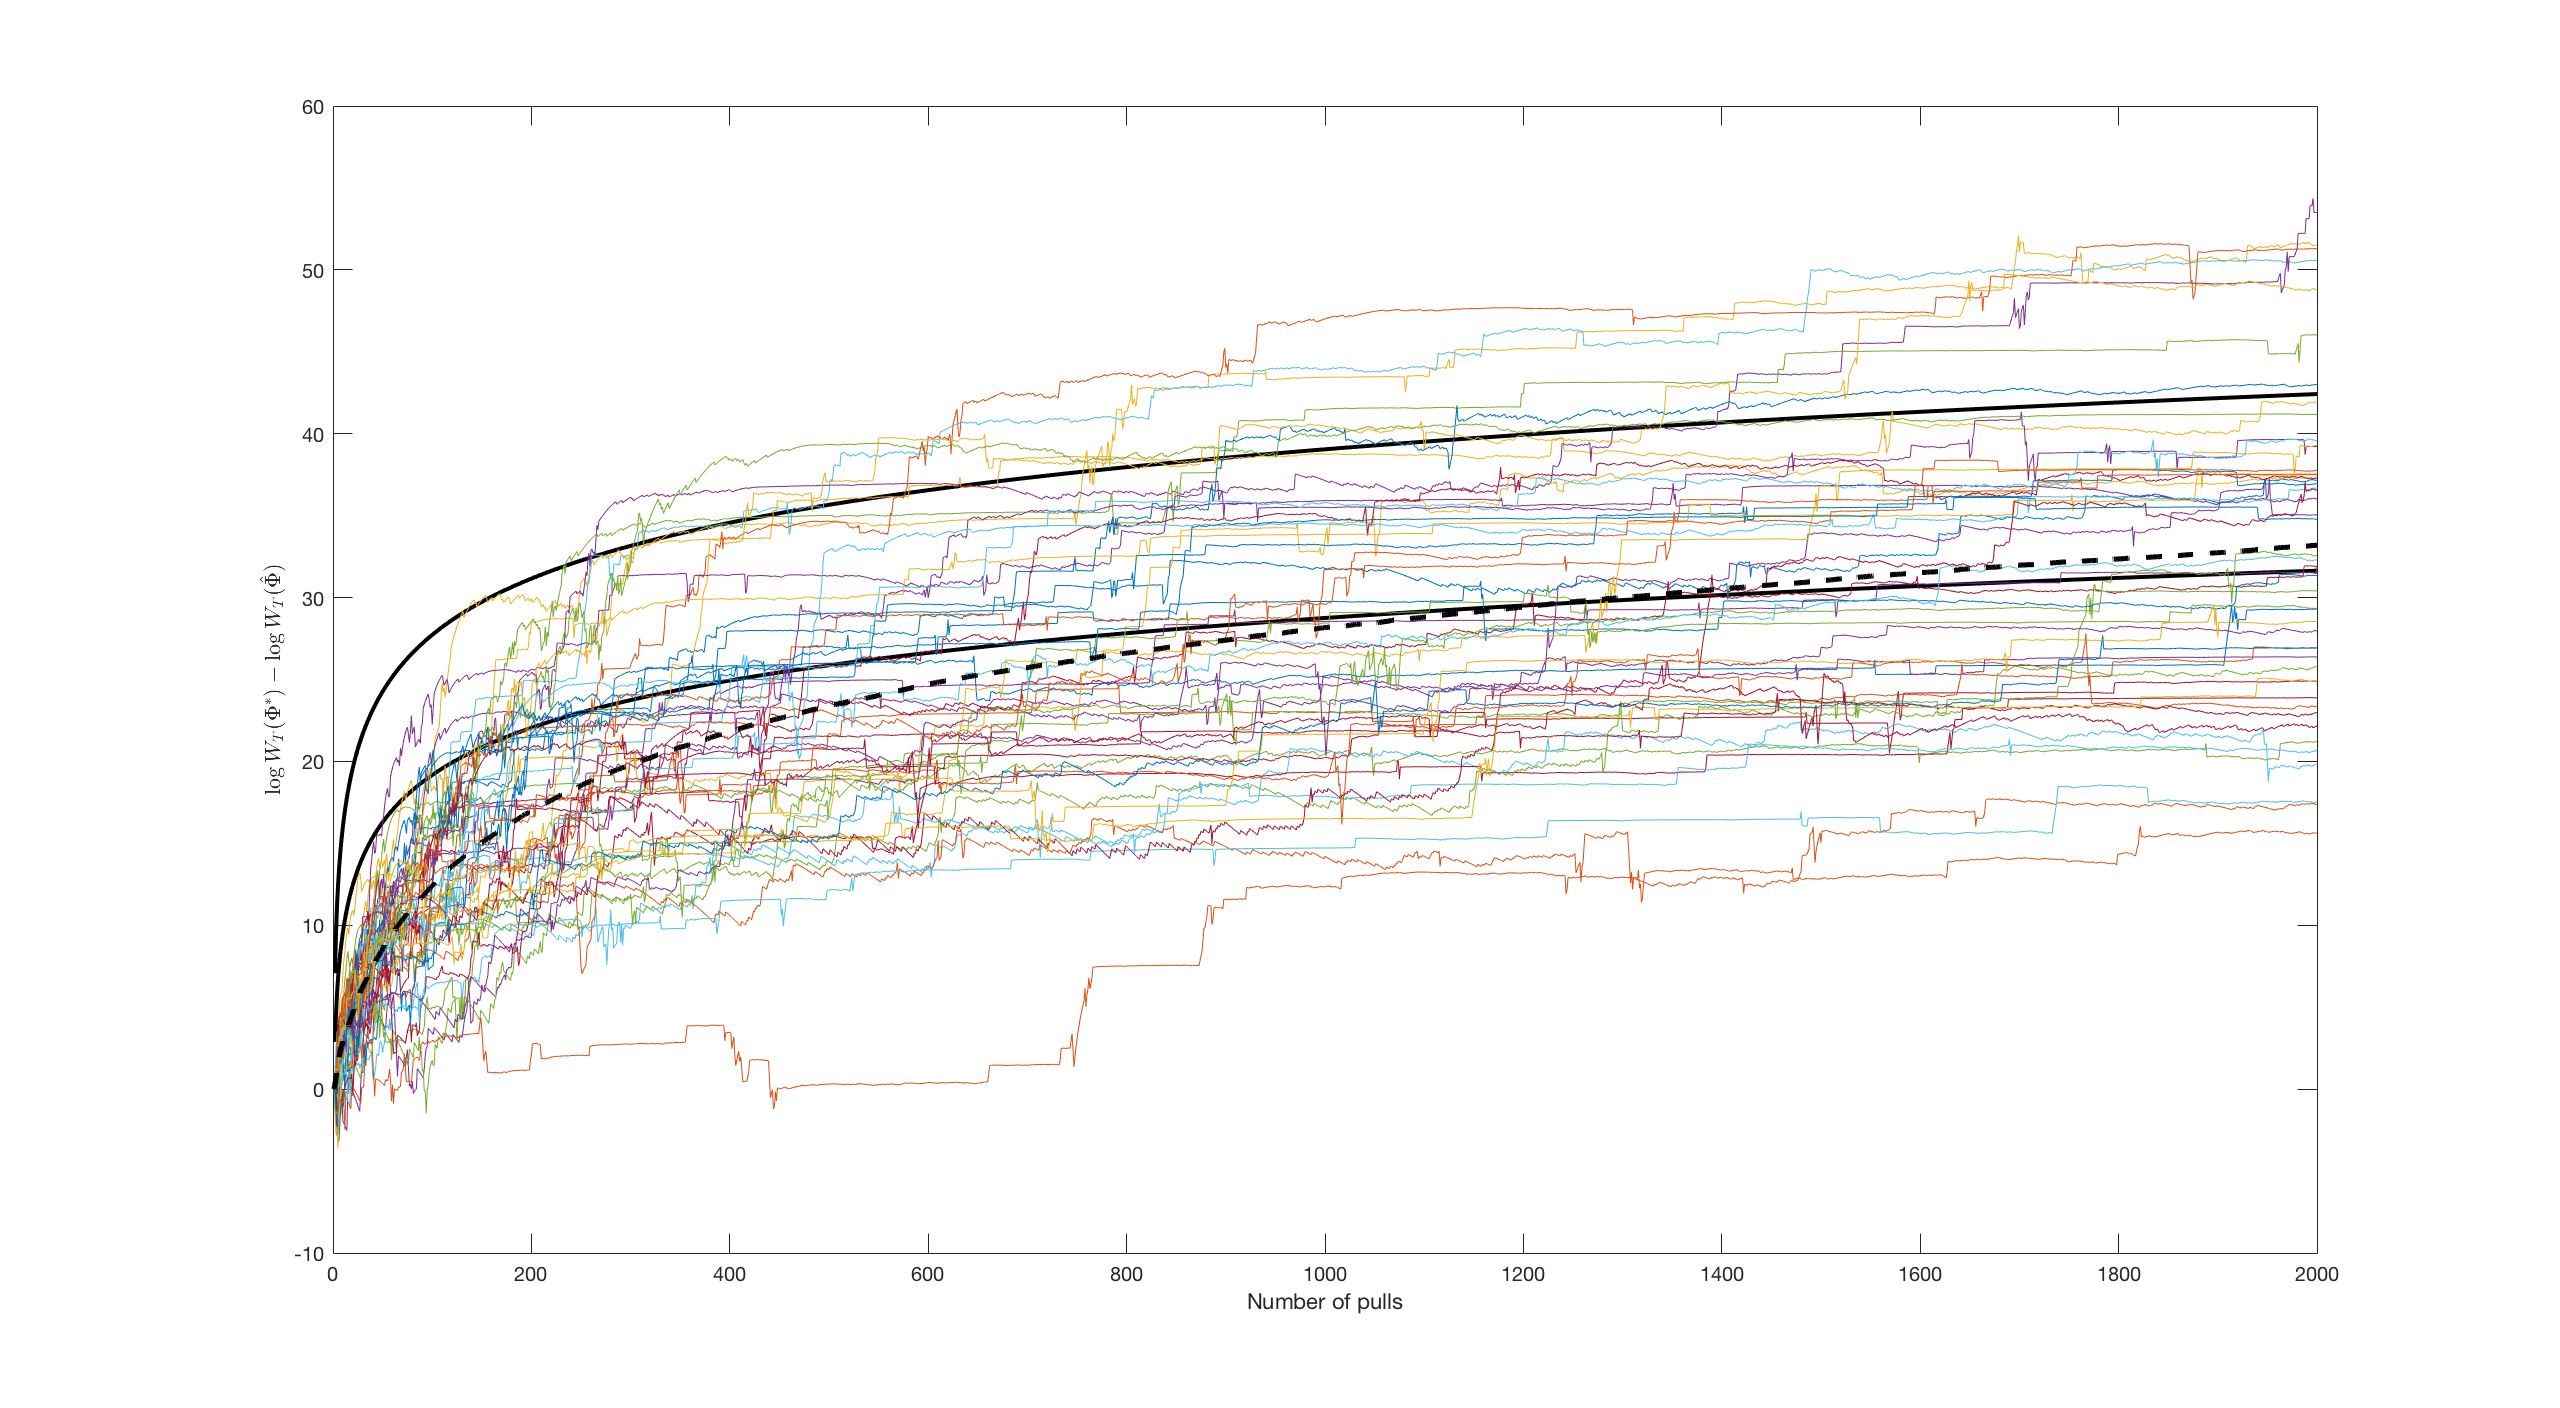
\includegraphics[width=\textwidth]{kelly_ucb_regret.png}
\caption{$\vec{p} = (0.4, 0.5, 0.6, 0.8)$. The top solid black curve is the expected regret bound\eqref{eq:kl_ucb_regret_bound}. The bottom solid black curve is the lower bound we get if we always use the Kelly bet (i.e. the regret only accumulates from choosing the wrong arm). The dashed black line is the mean regret of 2000 paths. The other plots are 50 randomly chosen regret paths.}
\label{fig:kelly_ucb_regret}
\end{figure}
\pagebreak
%TODO point out what is novel here

\bibliographystyle{abbrvnat}
\bibliography{kelly_ucb}

\end{document}
